% Many thanks to Andrew West for writing most of this file
% Main LaTeX file for CIS400/401 Project Proposal Specification
%
% Once built and in PDF form this document outlines the format of a
% project proposal. However, in raw (.tex) form, we also try to
% comment on some basic LaTeX technique. This is not intended to be a
% LaTeX tutorial, instead just (1) a use-case thereof, and (2) a
% template for your own writing.

% Ordinarily we'd begin by specifying some broad document properties
% like font-size, page-size, margins, etc. -- We have done this (and
% much more) for you by creating a 'style file', which the
% 'documentclass' command references.
\documentclass{sig-alternate}
 
% These 'usepackage' commands are a way of importing additional LaTeX
% styles and formattings that aren't part of the 'standard library'
\usepackage{mdwlist}
\usepackage{url}
\usepackage{tabularx}
\usepackage{tikz}
\usetikzlibrary{shapes,arrows}
\usepackage[export]{adjustbox}
\usepackage{lipsum,adjustbox}
\usepackage{listings}% http://ctan.org/pkg/listings
\lstset{
  basicstyle=\ttfamily,
  mathescape
}\begin{document} 

% We setup the parameters to our title header before 'making' it. Note
% that your proposals should have actual titles, not the generic one
% we have here.
\title{Verification of System FC in Coq}
\subtitle{Dept. of CIS - Senior Design 2014-2015\thanks{Advisors: Stephanie Weirich (sweirich@cis.upenn.edu), Richard Eisenberg (eir@cis.upenn.edu).}}
\numberofauthors{4}
\author{
  Tiernan Garsys \\ \email{tgarsys@seas.upenn.edu} \\ Univ. of Pennsylvania \\ Philadelphia, PA\\\\
  Lucas Pe\~{n}a \\ \email{lpena@seas.upenn.edu} \\ Univ. of Pennsylvania \\ Philadelphia, PA
  \and
  Tayler Mandel \\ \email{tmandel@seas.upenn.edu} \\ Univ. of Pennsylvania \\ Philadelphia, PA\\\\
  Noam Zilberstein \\ \email{noamz@seas.upenn.edu} \\ Univ. of Pennsylvania \\ Philadelphia, PA
}
\date{}
\maketitle

% Next we write out our abstract -- generally a two paragraph maximum,
% executive summary of the motivation and contributions of the work.
\begin{abstract}
  \textit{
Haskell's compiler, the Glasgow Haskell Compiler (GHC), generates code in GHC Core. The Coq proof assistant is used to verify substantial subset of System FC, the theoretical basis for GHC Core. A translation from the formal language to GHC Core, the concrete implementation of System FC that is used in GHC, will then be proven. The goal of verification is to prove that the evaluation semantics of System FC are sound.
  }

  \textit{
There are two main benefits to this project. First, the verification would provide assurance regarding the safety and accuracy of GHC. Second, and perhaps more importantly, it will provide foundation to verify other properties of GHC such as compiler optimizations.
 }

\textit{
(draft) Haskell is a statically-typed functional programming language that is commonly used for the compile-time guarantees about program behavior that its type system is believed to provide. Despite this usage, the type safety of  Haskell has not been formally proven. A foundation for a mechanized proof of Haskell's type safety is presented via a mechanized proof of the type safety of a substantial subset of System FC, the theor
 }
\end{abstract}

% Then we proceed into the body of the report itself. The effect of
% the 'section' command is obvious, but also notice 'label'. Its good
% practice to label every (sub)-section, graph, equation etc. -- this
% gives us a way to dynamically reference it later in the text via the
% 'ref' command, e.g., instead of writing `Section 1', you can write
% `Section~\ref{sec:intro}', which is useful if the section number
% changes.

\section{Introduction}
\label{sec:intro}


Content content content

\section{Background}
\label{sec:background}

\subsection{Haskell}
\label{sec:background-haskell}

Haskell is a functional programming language originally released in 1990. Haskell is a statically-typed language; the types of all expressions and variables are determined at compile-time via either type inference or explicit type annotations by the programmer. Haskell is strongly-typed, meaning that the usage of values in identifier declarations and functions must be consistent with the statically-declared types of these functions; Haskell will not implicitly convert values from one type to another in order to satisfy the static typing of the program. Haskell is also a purely-functional language; a function defined in Haskell is guaranteed not to have side-effects such as I/O or the mutation of data structures in the running environment unless this is explictly allowed by the programmer. 

The strong static typing of Haskell is attractive because it allows the programmer to make certain guarantees about the properties of his or her program at compilation, rather than runtime. Such guarantees include the guarantee that a function is never called with an invalid input type, or the guarantee that a function defines a behavior for null inputs. By determining these properties at compile-time, one can rule out entire classes of errors prior to ever running the program.

These advantages are founded on the believed type safety of Haskell. Type safety in a programming language refers to its resilience to type errors at runtime. In the context of a statically-typed language such as Haskell, type safety requires ensuring that the guarantees of behavior made at compile-time are preserved during program execution. Given type safety, one can be sure that the program does not exhibit undefined behavior (such as segmentation faults) during execution.

\subsection{GHC Core}
\label{sec:background-ghc-core}

The Glasgow Haskell Compiler, or GHC, is an optimizing compiler used to generate native executables from Haskell code. As with most compilers, GHC compiles programs in multiple phases, translating the source between various intermediate representations. These phases of compilation are outlined in Figure~\ref{fig:desgar}. Whereas a surface language, such as Haskell, is structured to be easy for humans to work with, these intermediate representations (also known as {\em core languages}) are designed to be easy for a compiler to modify and optimize.

In the first phase of compilation, Haskell code is type-checked and then converted into a desugared intermediate language called GHC Core. The conversion from Haskell to GHC Core involves adding explicit type annotations to all values (which, in Haskell, can be omitted by the programmer and subsequently inferred when type-checking), adding explicit type parameters to type declarations with polymorphic types, and assigning all identifiers globally-unique names. Once converted, GHC performs optimizations on the resulting GHC Core code before passing the program on to later stages of compilation.

\begin{figure}[h!]
  \centering
  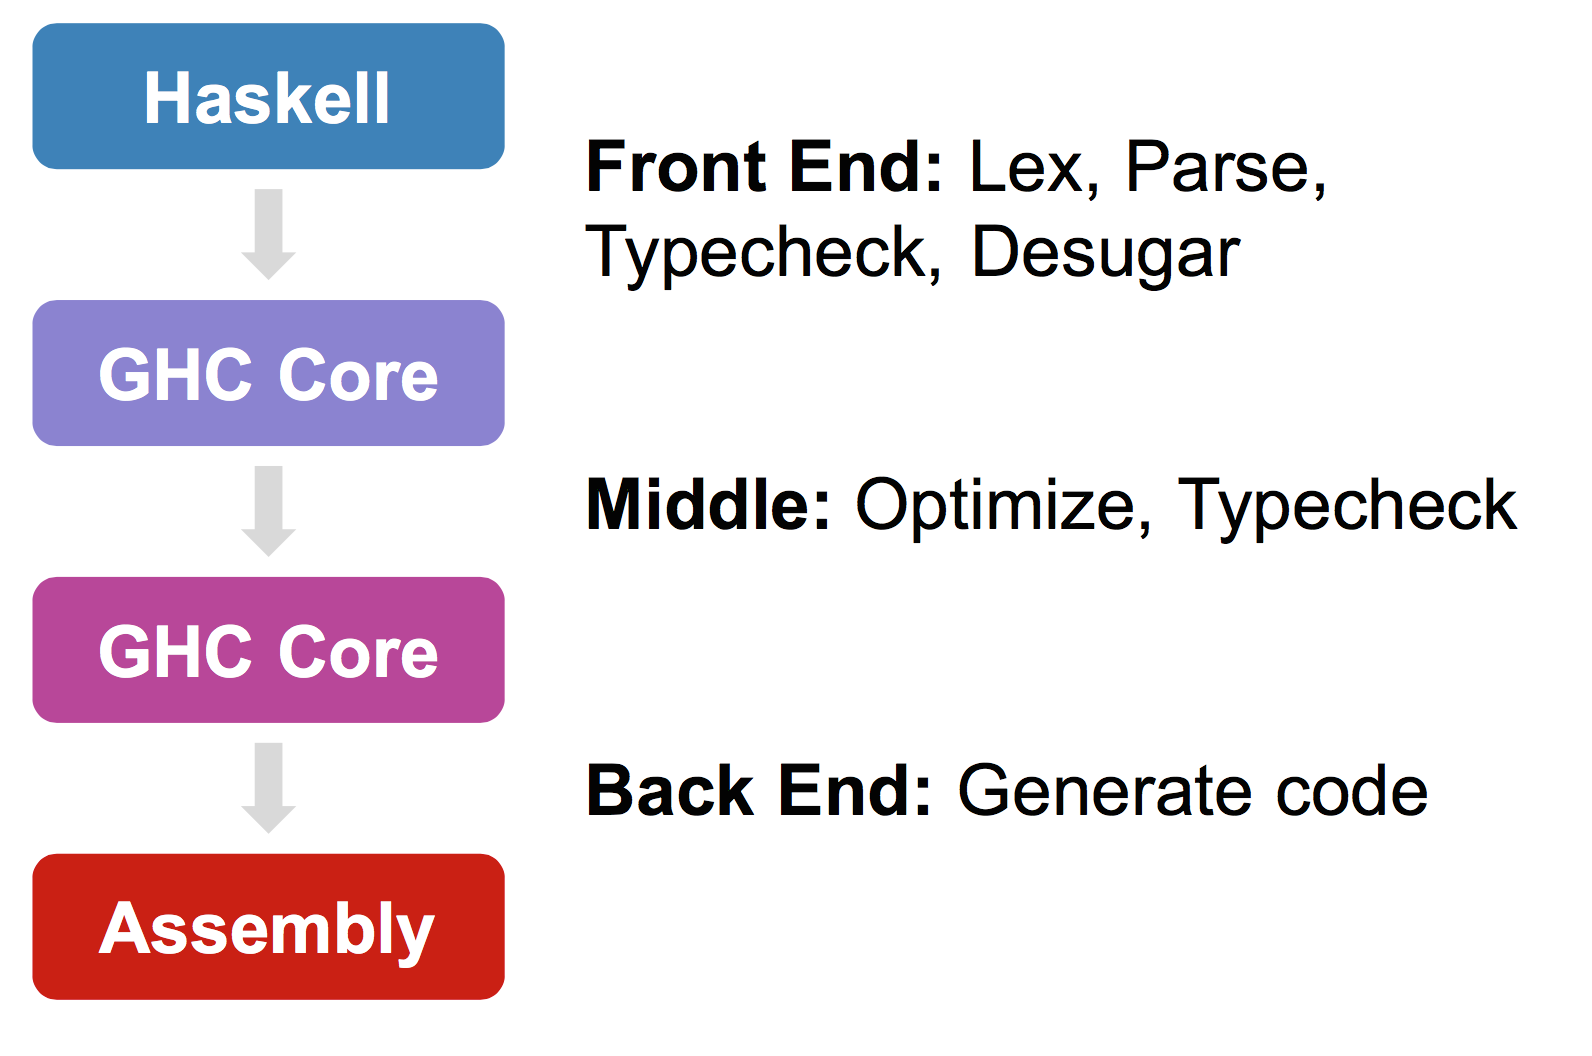
\includegraphics[max width=3in]{desgar.png}
  \caption{The GHC compilation process}
  \label{fig:desgar}
\end{figure}


\subsection{System FC}
\label{sec:background-fc}

GHC Core is an implementation of System FC, a programming language specification designed for use as a target language of Haskell. 

\subsection{Type Safety}
\label{sec:background-type-safety}

Should this even be here?!?

\section{Motivation}
\label{sec:motivation}

Content content content

\section{Related Work}
\label{sec:related-work}

Content content content

\section{Implementation}
\label{sec:implementation}

Content content content

\section{Results}
\label{sec:results}

Content content content

\section{Future Work}
\label{sec:future-work}

Content content content

\section{Ethical Considerations}
\label{sec:ethics}

lol

\section{Conclusion}
\label{sec:conclusion}

Content content content

% We next move onto the bibliography.
\bibliographystyle{plain} % Please do not change the bib-style
\bibliography{final_report}  % Just the *.BIB filename

% Here is a dirty hack. We insert so much vertical space that the
% appendices, which want to begin in the left colunm underneath
% "references", are pushed over to the right-hand column. If we looked
% hard enough, there is probably a command to do exactly this (and
% wouldn't need tweaked after edits).
\vspace{175pt}

\end{document} 
